\documentclass{article}
\usepackage{polski}
\usepackage[utf8]{inputenc}
\usepackage{natbib}
\usepackage{graphicx}
\usepackage{xcolor}
\usepackage{mathtools}
\usepackage{amssymb}
\usepackage[makeroom]{cancel}
\usepackage{hyperref}
\newcommand{\norm}[1]{\left\lVert#1\right\rVert}

\title{Sprawozdanie EX2}
\author{Jan Bronicki 249011}
\date{}


\begin{document}

\maketitle

\section{Podstawowe operacje na histogramie}

Rozciąganie jest przydatne przy obrazach, które nie wykorzystują całego zakresu histogramu. Operacja ta pozwala na powiększenie globalnego kontrastu w obrazie.

Wyrównanie polega na osiągnięciu bardzo płaskiego histogramu w całym zakresie który jest dostępny. Dzięki temu obrazy o małym skupieniu dostaną bardzo duży kontrast.

Model:

\begin{figure}[h!]
    \centering
    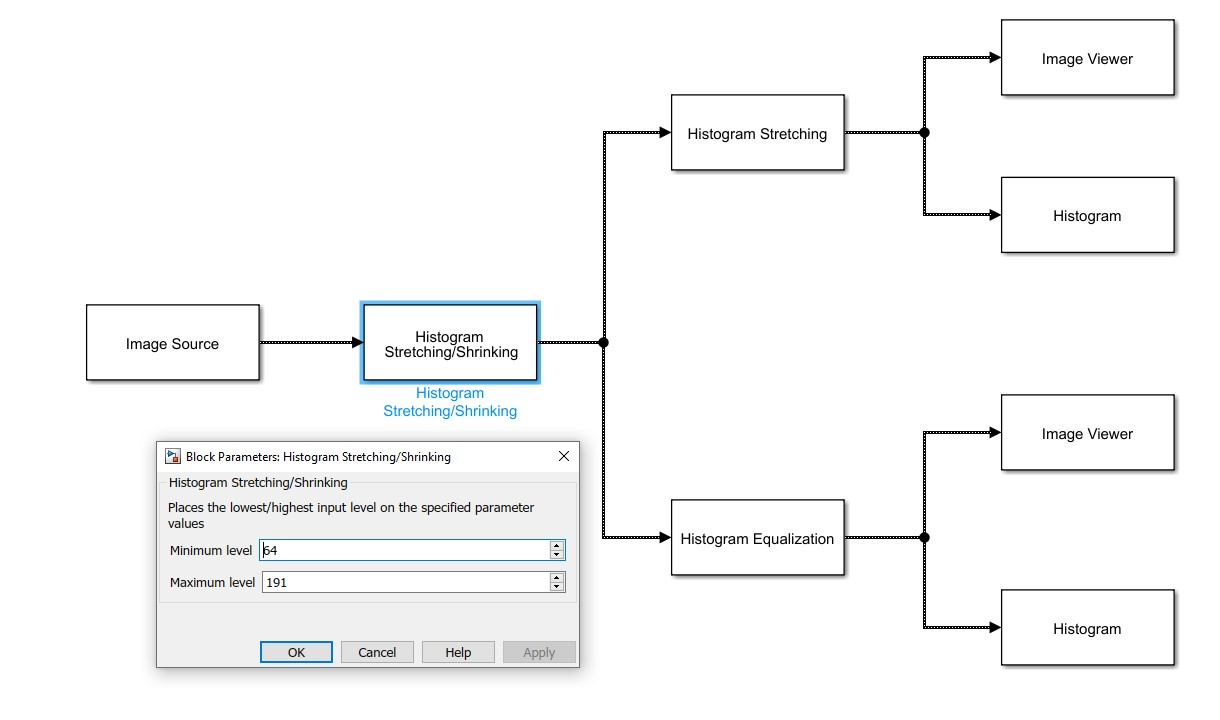
\includegraphics[scale=0.5]{zad1_model.jpg}
\end{figure}

\newpage

Oryginalny obraz w porównaiu z obrazezm o zawężonym histogramie:
\begin{figure}[h!]
    \centering
    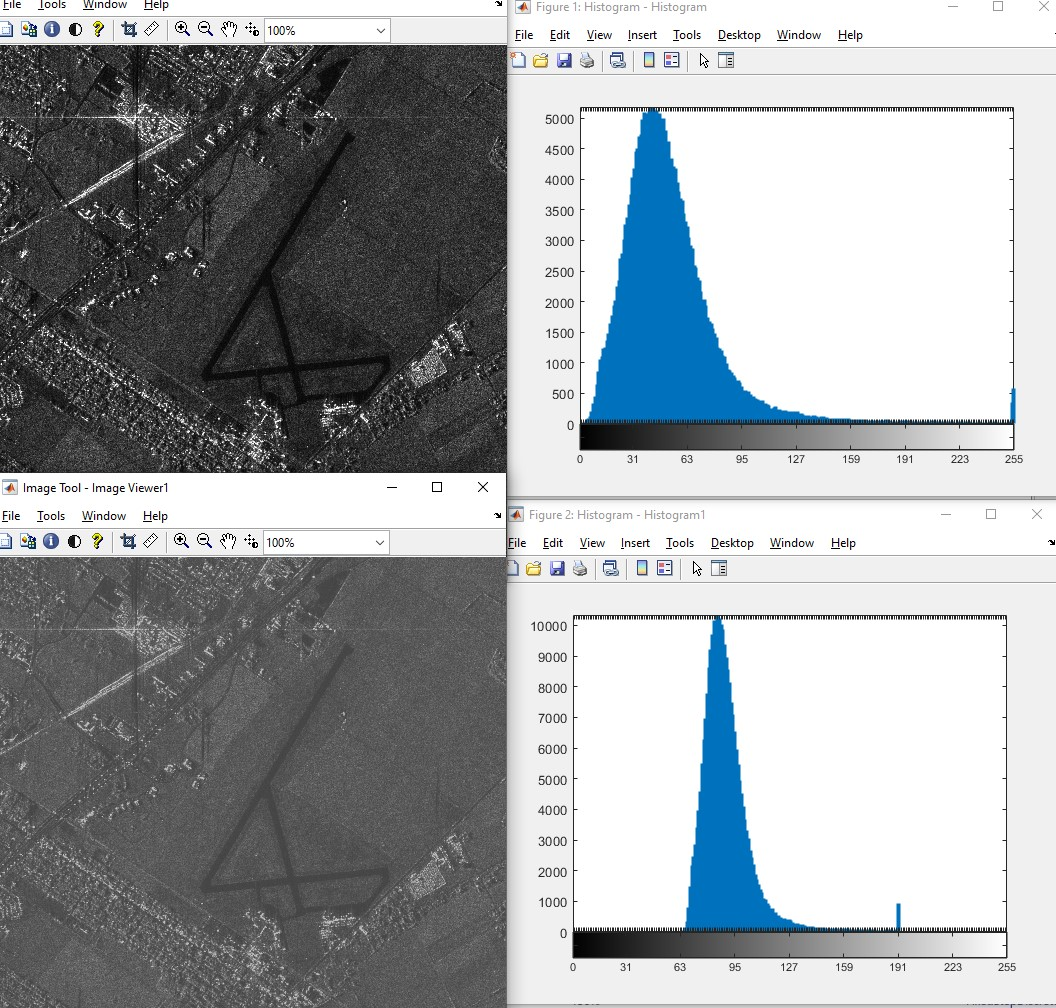
\includegraphics[scale=0.5]{zad1_bezeqsq.jpg}
\end{figure}

\newpage

Obrazy po wyrównaniu:

\begin{figure}[h!]
    \centering
    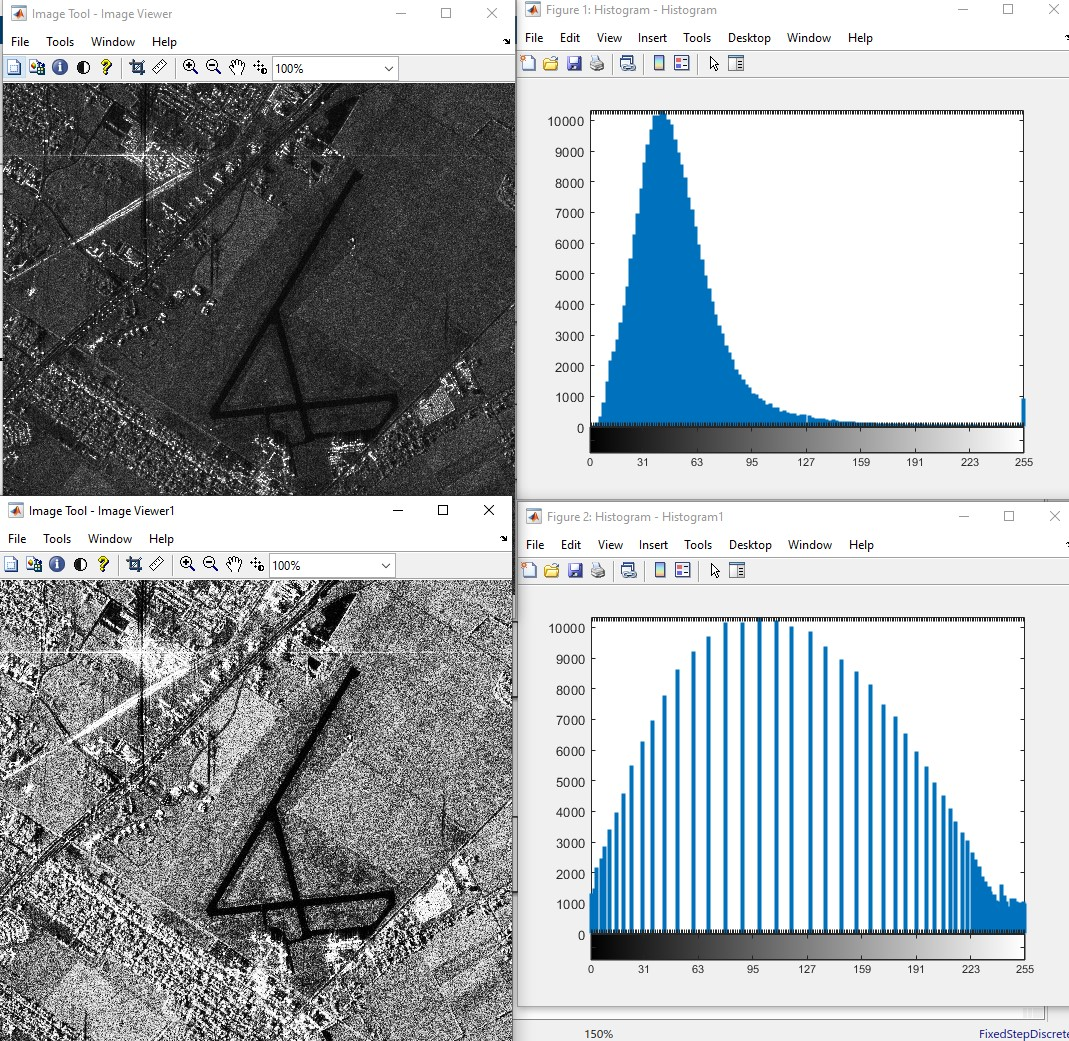
\includegraphics[scale=0.5]{zad1_porownanie1.jpg}
\end{figure}

\newpage

\section{Kwantyzacja po modyfikacji histogramu}

Kwantyzacja bez żadnych operacji przed nią rozjaśnia obraz, nie wpływa znacząco na kontrast, histogram zostaje zwężony.

Rozciągnięcie i kwantyzacja bardzo wpływają na kontrast dyn. obrazów, obszary wolnozmienne pozostają ujednolicone.

Wyrównanie i kwantyzacja nie tworzą kontrastu, aż tak mocnego jak rozciągnięcie, jednak pozwala na wyciągnięcie informacji z częsci wolnozzmiennych, pixele podobnych wartości zostają w wyniku procesu rozciągnięte na szerokości histogramu. W wyniku kwantyzacji przypisane do różnych widocznie różnych
wartości, dzięki czemu możemy zdobyć nowe informacje.



Model:

\begin{figure}[h!]
    \centering
    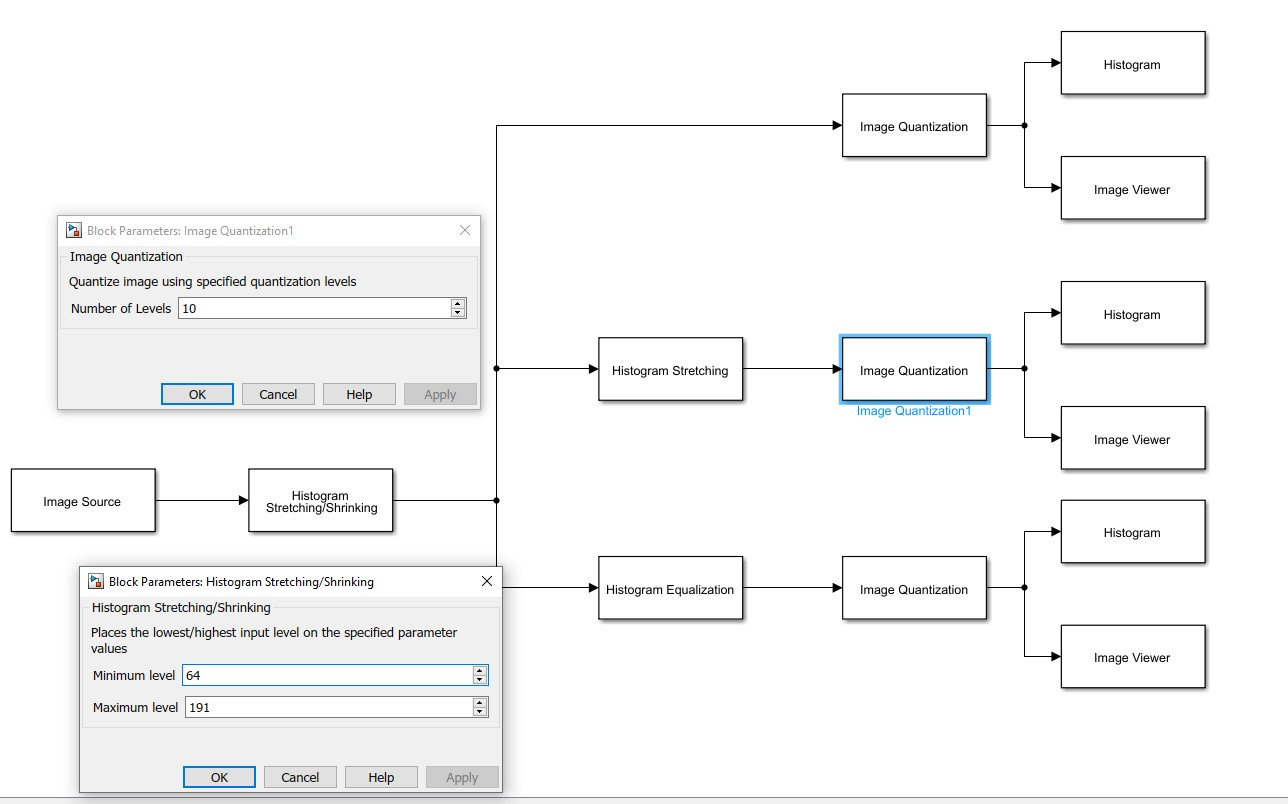
\includegraphics[scale=0.5]{zad2_model.jpg}
\end{figure}

\newpage

Obraz oryginalny oraz obraz o zwężonym histogramie poddany kwantyzacji:

\begin{figure}[h!]
    \centering
    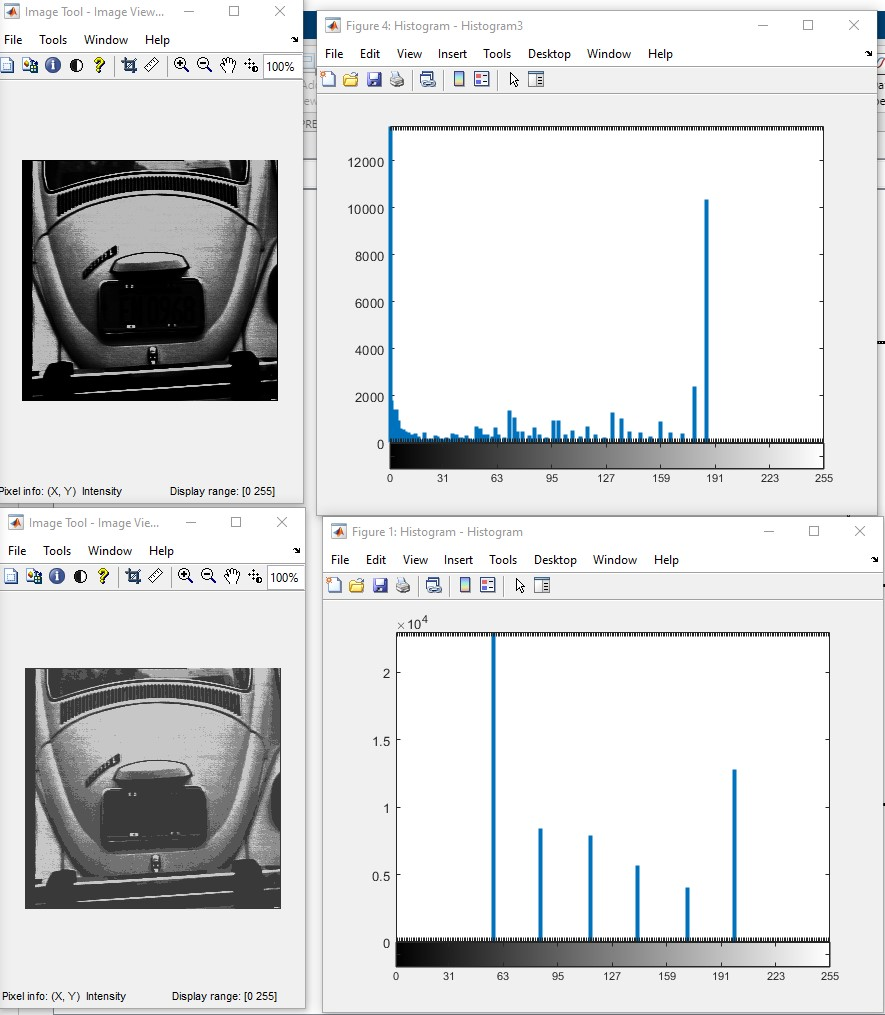
\includegraphics[scale=0.5]{zad2_a.jpg}
\end{figure}

\newpage

Obrazy po wyrównaniu/rozciągania i kwantyzacji:


\begin{figure}[h!]
    \centering
    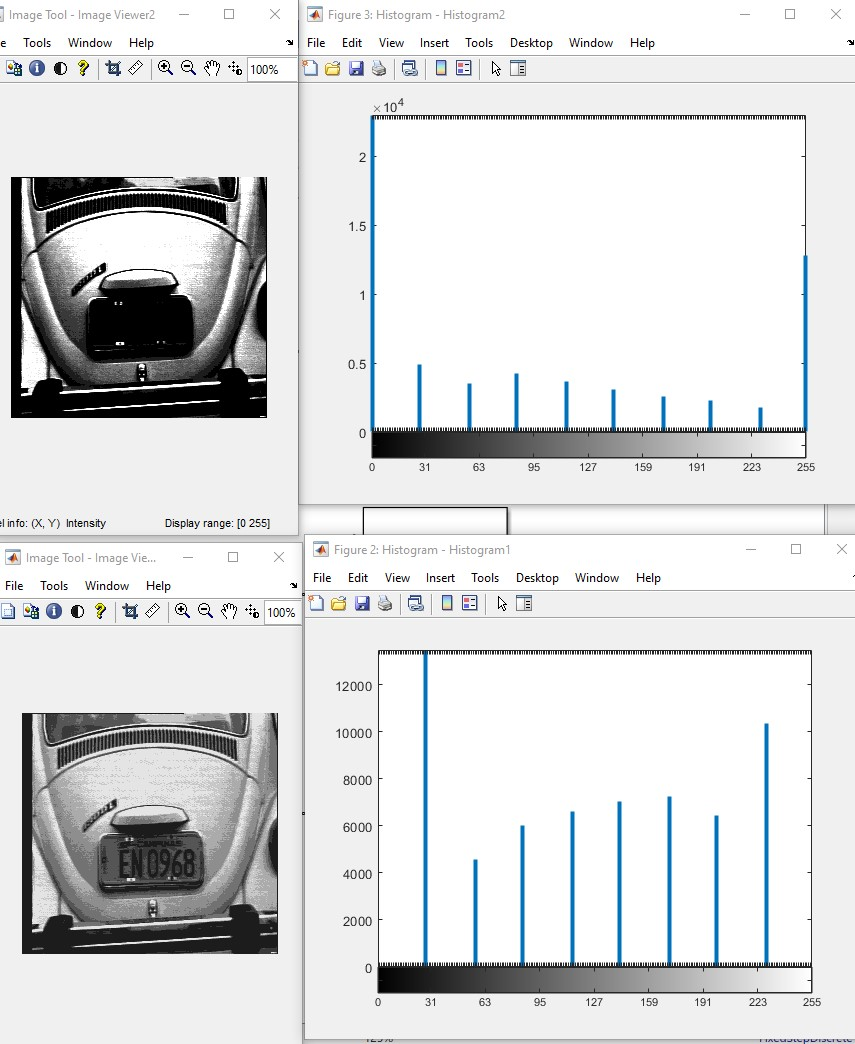
\includegraphics[scale=0.5]{zad2_b.jpg}
\end{figure}


\end{document}